\chapter{Pulse shape simulation}
\label{cha:pss}
How segmentation can be used to distinguish between single- and
multi-segment events and how to use this information was described in
chapters~\ref{cha:photon} and~\ref{cha:neutron}.  However, as was
shown in Fig.~\ref{fig:ph:eve}, (1) there are some multi-site events
which are confined to one segment and (2) there are some single-site
events that happen on the boundary between two segments. If the
signal is identified with single-segment events, events from
category~(1) are counted erroneously as signal and events form
category~(2), \textit{boundary events}, are rejected erroneously,
because the energy deposited is shared between segments.

The analysis of the electrical pulses associated with the events
(pulse shape analysis) can help with both problems\footnote{Pulse
shape analysis can also help with several other aspects: rejection of
background from $\alpha$-particle and neutron interactions with
detectors, Compton continuum suppression\cite{comcon}, detection of
crystal structure~\cite{agata}, etc.}. For category (1) the time
development of the pulse can reveal a multi-site event while for
events in category (2) a close to equal strength and time development
of the two pulses can reveal its true single-site structure.
Concerning (1), previous studies \cite{Kev07} indicate that pulse
shape analysis can provide an extra suppression factor of 1.3 beyond
the suppression achieved through segment information alone. These
studies were limited by the lack of knowledge about the development of
the pulses in the detector and its support system.

Pulses resembling the ones expected for the $0\nu\beta\beta$ signal
are usually collected using photon induced events with a similar event
topology. Two data samples commonly used are (A) double escape peak
(DEP) events and (B) single Compton scattering
events\cite{scoms}. However, the double escape peaks are normally not
located near the Q-value of $^{76}$Ge $0\nu\beta\beta$ decay. In
addition, the events from the peak are not uniformly distributed
throughout the detector crystal \cite{major}.  Events from single
Compton scattering could, in principle, be selected to overcome these
restrictions. However, it is intrinsically difficult to collect
sufficiently large such samples.  Therefore, it is essential to
supplement the data with simulated pulses from a reliable simulation.

The physics models used for the drift of electrons and holes inside
germanium crystals were established by L. Mihailescu \textit{et
al.}\cite{miha} and B. Bruyneel \emph{et al.} \cite{bart},
respectively. The implementation of these models for Siegfried-like
detectors is described in detail in this chapter.


\section{Procedure}
\label{sec:pss:proc}
The procedure to simulate pulse shapes \cite{agata} is as follows:
\begin{enumerate} 
\item Simulate the interactions of particles with germanium using
Geant4 to get the spatial distribution and the energy deposits of the
interactions (hits);
\item Group hits if they are closer to each other than 1~mm. The
position of the new hit is the barycenter of the energies of the
original hits. The energy of the new hit is the sum of the energies of
the original hits.
\item Calculate the number of electron-hole pairs, $n$, created by the
hit with energy $E_{\text{hit}}$: $n = E_{\text{hit}} /
E_{\text{pair}}$, where the pair energy $E_{\text{pair}} = 2.95$~eV;
\item Calculate the electrical field and the weighting
potentials\,\cite{Gat82, Rad88, He00} in the detector according to the
high voltage applied and the spatial distribution of the impurity. The
calculation of the fields and weighting potentials is done only
once. The results are saved for interpolation later;
\item Calculate the drift velocities of the charge carriers taking
into account the effect of the crystal structure;
\item Calculate the trajectory of the drift from the interaction point
to the boundary of the crystal;
\item Calculate the time development of the charges induced in the
electrodes i.e. the pulses \cite{igex}. A dominant pulse is seen in
the electrode of the segment hit. However, other electrodes also show
pulses, so called mirror pulses, which also have to be simulated.
\item Add to the simulated pulses the effects from the electronics
such as noise, bandwidth limit, and shaping, etc.
\end{enumerate} 
MaGe, the object-oriented simulation package co-developed by the GERDA
and Majorana MC groups described in Sec.~\ref{sec:ph:sim} covers the
complete procedure. Step 5-7 were developed as part of this
thesis. The calculation of the electric fields and potentials is
described in Sec.~\ref{sec:pss:field}, the calculation of the drift
velocities of the charge carriers in Sec.~\ref{sec:pss:drift}.
 
 
\section{Electric and weighting fields} 
\label{sec:pss:field} 
The electric field $\mathbf{E}$ could, in principle, be calculated by
solving analytically Poisson's equation $\nabla \cdot \mathbf{E} =
\frac{\rho}{\epsilon}$ as described in Sec.~\ref{sec:det:field}. It is
more practical to numerically calculate the potential field
$\varphi$. The electric field $\mathbf{E}$ is then obtained using
$\mathbf{E} = - \nabla \varphi$. Since true coaxial detectors are
used, it is convenient to use cylindrical coordinates, $r, \phi, z$:
\begin{equation} 
\frac{1}{r} \frac{\partial \varphi}{\partial r} + \frac{\partial^{2} \varphi}{\partial r^{2}} + \frac{1}{r^{2}} \frac{\partial^{2} \varphi}{\partial \phi^{2}} + 
\frac{\partial^{2} \varphi}{\partial z^{2}} = - \frac{1}{\epsilon_{0} 
\epsilon_{R}} \rho, 
\label{eq:pss:pocyl} 
\end{equation} 
where $\varphi$ and $\rho$ are functions of $r, \phi, z$;
$\epsilon_{0}$ and $\epsilon_{R}$ are the dielectric constants in
vacuum and germanium, respectively.
 
The electric field distribution inside the germanium crystal is quite
sensitive to the impurity density. Figure~\ref{fig:pss:rho} shows the
strength of the electric field as a function of $r$ with the bias
voltage fixed at 3~kV.  A change of the impurity density by one order
of magnitude changes the electric field dramatically. Even a factor
three difference, usually allowed between top and bottom for a
commercial detector, has a very significant effect.

 
\begin{figure}[htbp] 
\centering 
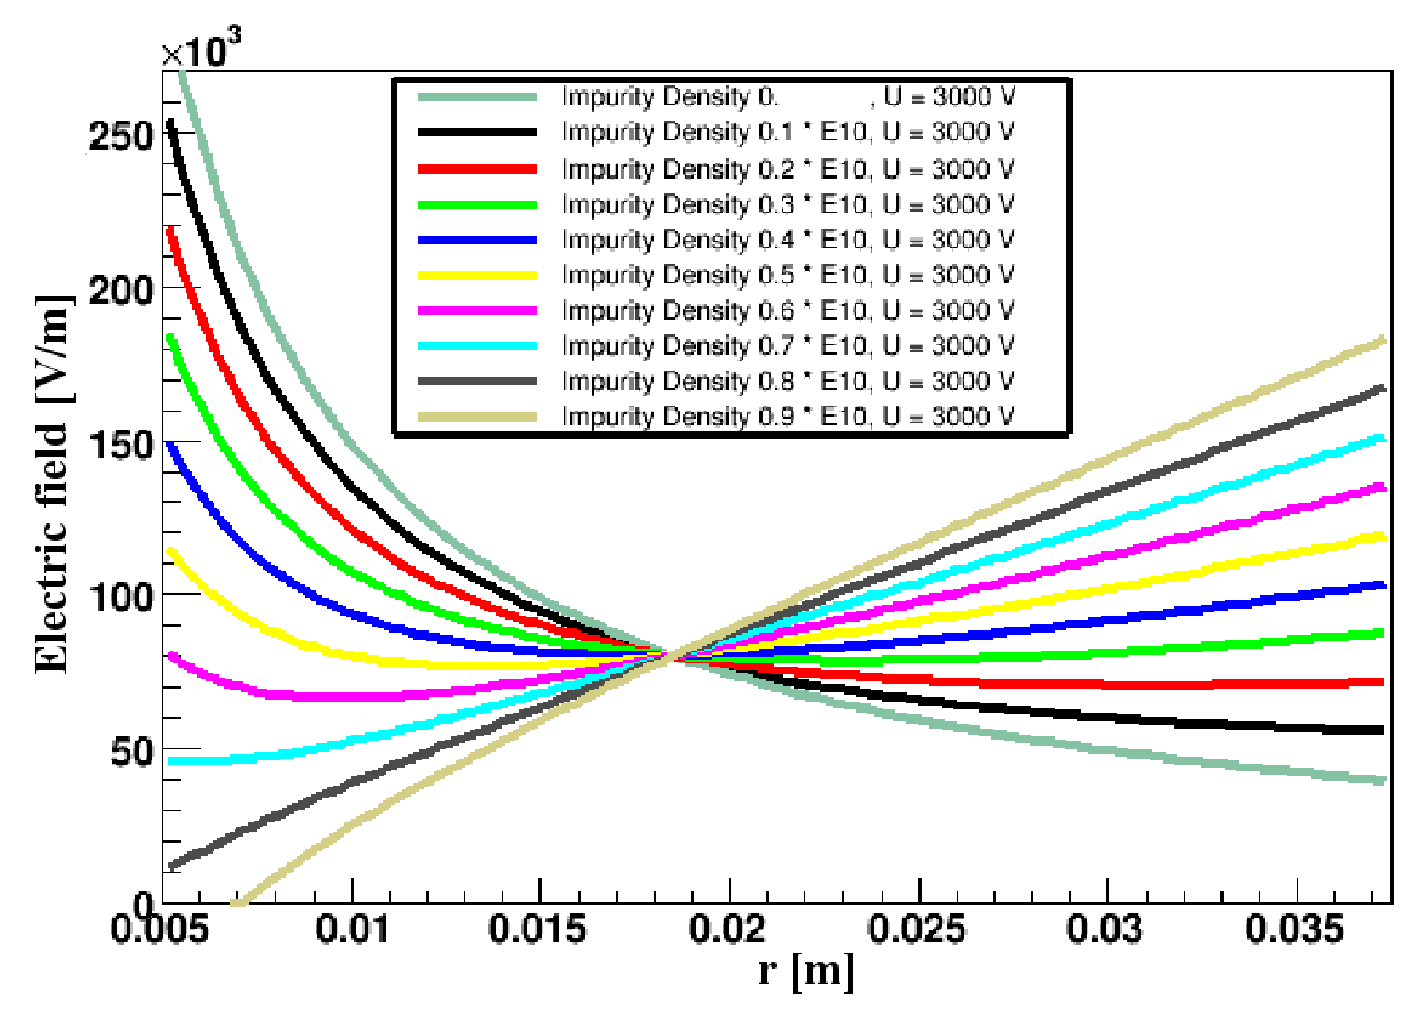
\includegraphics[width=0.7\textwidth]{rho} 
\caption{Strength of the electric field as a function of the
cylindrical coordinate $r$ for impurity densities between 0 and $0.9
\times 10^{-10}$/cm$^{3}$.}
\label{fig:pss:rho} 
\end{figure} 
 
The weighting fields and potentials are calculated in the same way to
determine the signals induced in the electrodes using Shockley-Ramo's
Theorem \cite{Gat82, Rad88, He00} as described in
Sec.~\ref{sec:det:ramo}.
 
 
\section{Drift of charge carriers} 
\label{sec:pss:drift} 
 
\subsection{Mobility} 
\label{sec:pss:mobi} 
The electrons and holes drift to the electrodes of the detector. The
mobilities of electrons $\mu_{e}$ and holes $\mu_{h}$ as defined in
Sec.~\ref{sec:det:struc} change with the temperature of the germanium
crystal. If the temperature of electrons and holes\footnote{If the
velocities of a group of electrons or holes follow a Maxwell-Boltzmann
distribution, their temperature is defined as the temperature of that
distribution.} do not differ much from the temperature of the crystal
lattice, the drift velocity $\mathbf{v}_{e/h}$ is simply proportional
to the electrical field and the crystal structure has no
influence. The mobility in this case is just a number,$\mu_{0}$. As
germanium detectors are operated at $\approx 100$~K, the electrons and
holes are hotter than the crystal lattice. The mobility in this case
depends on the crystal orientation and is a complex tensor. The drift
trajectory, hence, is not always parallel to the electric field.
 
Germanium has the same crystalline structure as silicon and diamond,
\textit{i.e.} a face-centered cubic (FCC) structure: each atom is at
the center of a regular tetrahedron and is surrounded by four atoms as
shown in Fig.~\ref{fig:pss:xtal}.
 
\begin{figure}[tbhp] 
\centering 
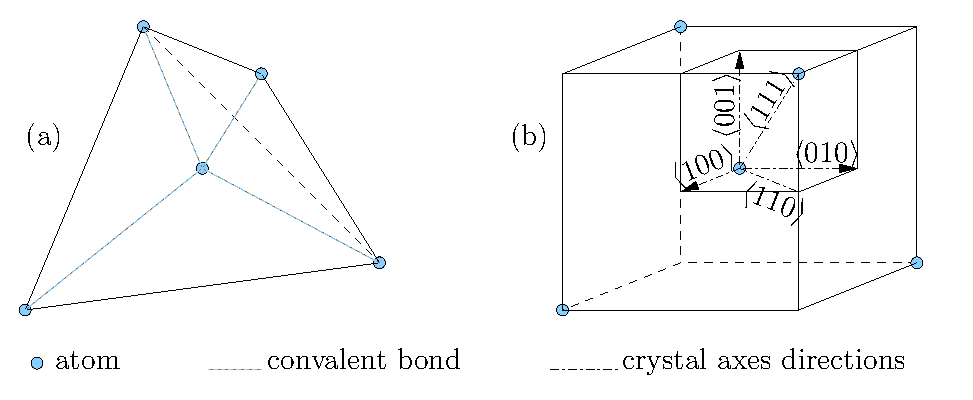
\includegraphics[width=0.8\textwidth]{xtalStruc}   
\caption{Structure of germanium crystals: (a) basic configuration and
(b) definition of crystal axes.}
\label{fig:pss:xtal} 
\end{figure} 
 
If the electric field lines are parallel to any of the three principal
crystallographic axes $\langle 100 \rangle$, $\langle 110 \rangle$ and
$\langle 111 \rangle$, the charge carriers will drift along the
electric field because of the symmetric structure of the germanium
crystal. In this case the drift velocity only depends on the strength
of the electric field. Measurements of the drift velocities along the
axes $\langle 100 \rangle$ and $\langle 111 \rangle$ with electric
field parallel to them were performed and the data can be fitted well
by the following parametrization \cite{Kno99}:
\begin{equation} 
\label{eq:pss:para} 
v = \frac{\mu_{0}E}{[1+(\frac{E}{E_{0}})^{\beta}]^{1/\beta}} - \mu_{n}E, 
\end{equation} 
where $E, v$ are the magnitudes of the electric field and drift
velocity, respectively, $\mu_{0}, \mu_{n}, E_{0}$ and $\beta$ are
parameters to be determined by fitting. The parameter $\mu_{0}$
represents a simple linear relation between $v$ and $E$. A deviation
from this linear relation occurs at low temperatures
($\approx$100~K). It is modeled through the par;ameters $E_{0}$ and
$\beta$. Mihailescu \textit{et al.} \cite{miha} added the term
$\mu_{n}E$ for electric fields stronger than 300~V/mm to account for
the \emph{Gunn effect} observed by Ottaviani \textit{et al.}
\cite{otta}. This effect is irrelevant here as our detectors are
operated at field strengths well below 300~V/mm. The values of the
parameters of the fit to the experimental data are listed in
Table~\ref{tab:pss:pars}. They are an important input for the
simulation presented here.
 
\begin{table}[tbhp] 
\centering 
\caption{Parameters for the experimental drift velocities in the $\langle111\rangle$ and $\langle 100 \rangle$ directions (taken from Ref.~\cite{bart}).} 
\label{tab:pss:pars} 
\begin{tabular*}{\textwidth}{ccccccc}\hline\hline 
Reference & Carrier & Direction & $\mu_{0} \left[ \frac{\mbox{cm}^{2}}{\mbox{V}\cdot\mbox{s}} \right]$ & $E_{0} \left[ \frac{\mbox{V}}{\mbox{mm}} \right]$ & $\beta$ & $\mu_{n} \left[ \frac{\mbox{cm}^{2}}{\mbox{V}\cdot\mbox{s}} \right]$ \\\hline 
& Electrons & $\langle111\rangle$ & 40180 & 49.3 & 0.72 & 589 \\ 
Ref.~\cite{miha}& & $\langle100\rangle$ & 42420 & 25.1 & 0.87 & 62\\ 
& Holes & $\langle111\rangle$ & 107270 & 10.0 & 0.58 & 0 \\ 
& & $\langle100\rangle$ & 66333 & 18.1 & 0.744 & 0 \\\hline 
& Electrons & $\langle111\rangle$ & 38536 & 53.8 & 0.641 & 510 \\ 
Ref.~\cite{bart}& & $\langle100\rangle$ & 38609 & 51.1 & 0.805 & -171\\  
& Holes & $\langle111\rangle$ & 61215 & 18.2 & 0.662 & 0 \\ 
& & $\langle100\rangle$ & 61824 & 18.5 & 0.942 & 0 \\\hline\hline 
\end{tabular*} 
\end{table} 
 
Figure~\ref{fig:pss:vvse} shows the drift velocities of electrons (a, c) and holes (b, d) along the principal crystal axes as functions of electric field in the range of [7,500]~V/mm. The drift velocities along the $\langle 100 \rangle$ and $\langle 111 \rangle$ axes were calculated according to Eq.~\ref{eq:pss:para}. The input parameters provided in Ref.~\cite{miha} (\cite{bart}) were used for Fig.~\ref{fig:pss:vvse}a and b (c and d). 
The drift velocity in any direction 
can be derived from the velocities along  the 
$\langle 100 \rangle$ and $\langle 111 \rangle$ axes.
The details of the calculation are described in the following sections. 
 
\begin{figure}[tbhp] 
\centering 
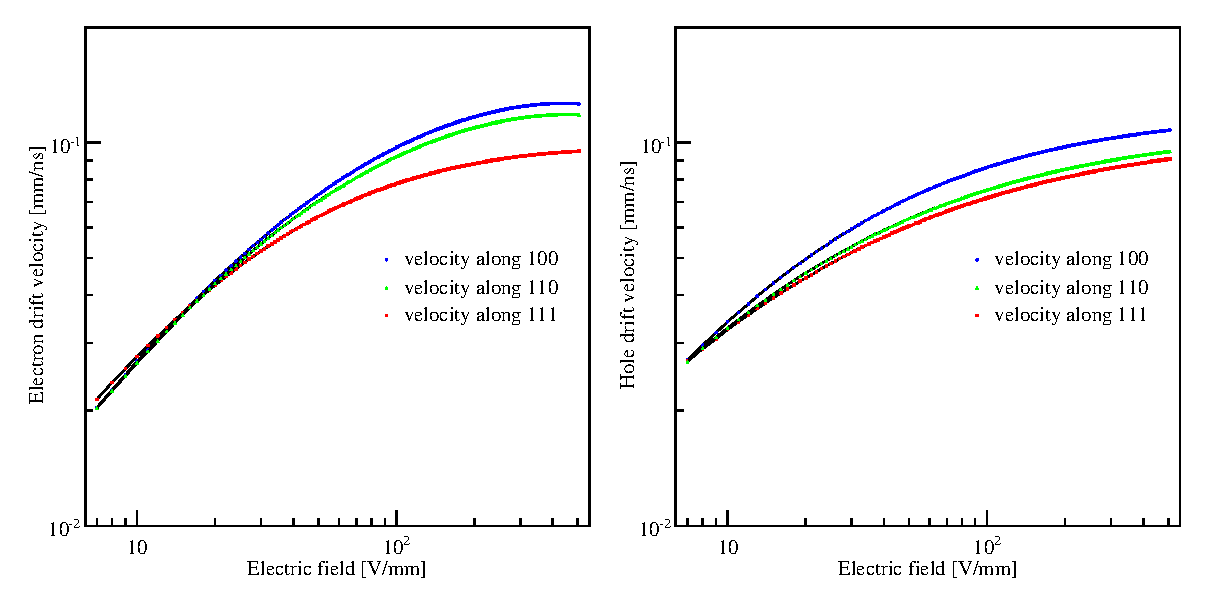
\includegraphics[width=\textwidth]{VvsElucian} \\\hfil 
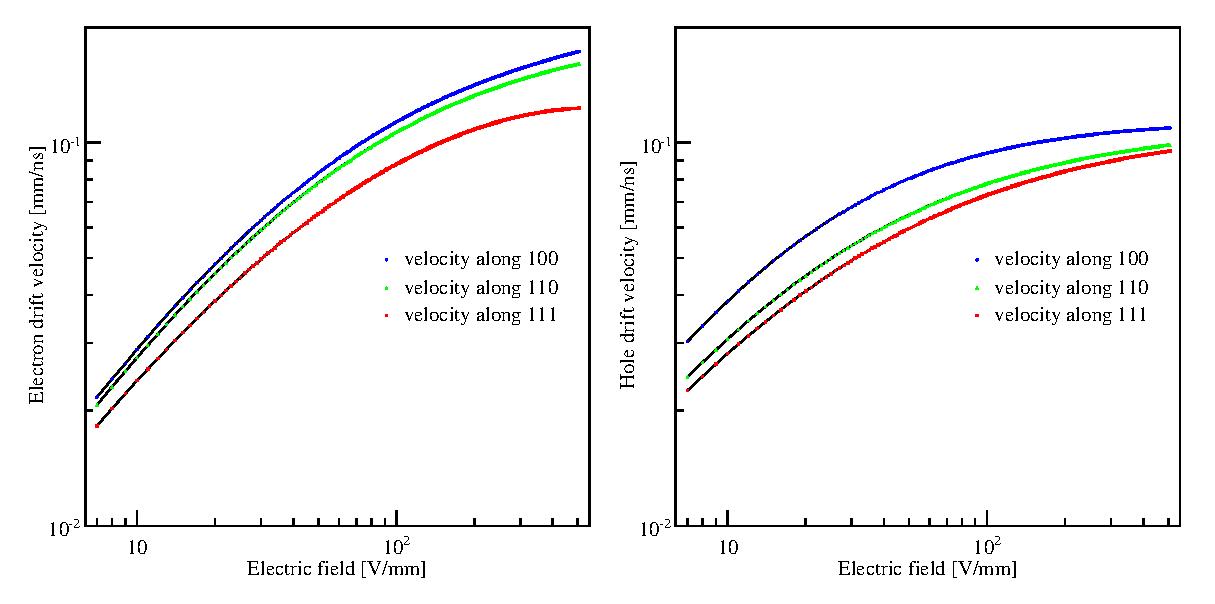
\includegraphics[width=\textwidth]{VvsEbart} 
\caption{Drift velocities of electrons (a, c) and holes (b, d) along
the principal crystal axes as functions of electric field in the range
of [7,500]~V/mm. Velocities along the axes $\langle 100 \rangle$ and
$\langle 111 \rangle$ were calculated according to
Eq.~\ref{eq:pss:para}: (a) and (b), the input parameters provided in
Ref.~\cite{miha} were used; (c) and (d), the input parameters provided
in Ref.~\cite{bart} were used. The velocities along the $\langle 110
\rangle$ axis are predicted according sections~\ref{sec:pss:elec}
and~\ref{sec:pss:hole}.}
\label{fig:pss:vvse} 
\end{figure} 
 
\subsection{Coordinate systems} 
\label{sec:pss:xyz} 
Two different coordinate systems are important for the
calculation. The first one is defined by the crystal axes $\langle 100
\rangle$, $\langle 010 \rangle$ and $\langle 001 \rangle$. The second
one, indicated as $xyz$ in Fig~\ref{fig:pss:coo}, is used in
Geant4. The cylindrical detectors are produced with their geometrical
middle axis, $z$, aligned to the crystal axis $\langle 001
\rangle$. The transformation between the two coordinate system, hence,
only depends on the angle between the $\langle 110 \rangle$ and the
y-axis, $\phi_{110}$.
\begin{SCfigure}[][t!] 
\centering 
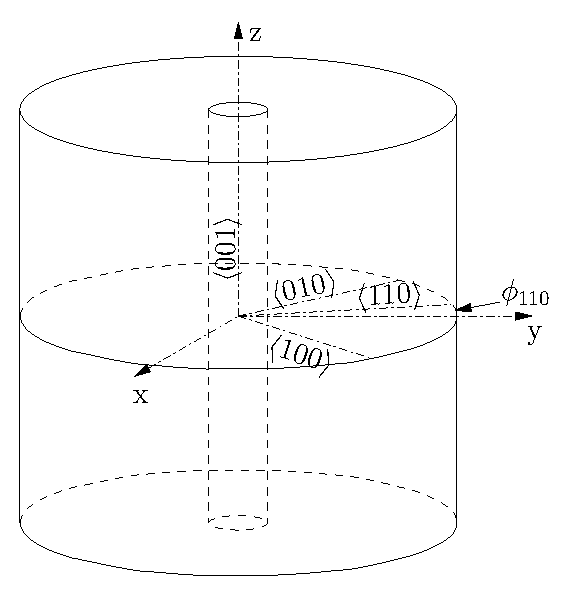
\includegraphics[width=0.4\textwidth]{coordins}   
\caption{The relation between the coordinates $xyz$ used in Geant4 and
the crystal axes $\langle 100 \rangle$, $\langle 010 \rangle$ and
$\langle 001 \rangle$.}
\label{fig:pss:coo} 
\end{SCfigure} 
 
\subsection{Electron drift velocity} 
\label{sec:pss:elec} 
The conduction band in a germanium crystal reaches its minimal
potential in regions around the four equivalent $\langle 111 \rangle$
axes. The equipotential surfaces in these regions have ellipsoidal
shapes as shown in Fig~\ref{fig:pss:valley}.
\begin{SCfigure}[][b!] 
\centering 
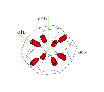
\includegraphics[width=0.4\textwidth]{valleys}   
\caption{Minimal potential regions in the conduction band along four
equivalent $\langle 111 \rangle$ axes, where the probability density
of electrons is dominant (taken from Ref.\cite{bart}).}
\label{fig:pss:valley} 
\end{SCfigure} 
These regions are characterized by valleys in the conduction band
which can easily be populated by free electrons. The electrons have a
high mobility and are strongly accelerated by the electric field
applied.  The probability density of conduction band electrons in
other regions is very small. If it is neglected, the dependence of the
electron drift velocity $\mathbf{v}_{e}$ on the applied electric field
$\mathbf{E}$ can be written as
\begin{equation} 
\label{eq:pss:ed} 
\mathbf{v}_{e}(\mathbf{E}) = \mathcal{A}(E) \sum_{j} \frac{n_{j}}{n} \frac{\gamma_{j}\mathbf{E_{0}}}{\sqrt{\mathbf{E_{0}}\gamma_{j}\mathbf{E_{0}}}}, \mbox{ with } j=1,2,3,4, 
\end{equation} 
where the coefficient $\mathcal{A}$ is a function of $E=|\mathbf{E}|$
and the temperature; $\mathbf{E_{0}}$ is the normalized electric field
vector; $n_{j}/n$ is the fraction of the carriers (in this case,
electrons) in the $j$-th $\langle 111 \rangle$ valley and $\gamma_{j}$
is the effective mass tensor for the electrons in the $j$-th $\langle
111 \rangle$ valley. Local coordinates,
$x^{\prime}y^{\prime}z^{\prime}$, are defined as shown in
Fig.~\ref{fig:pss:axes}. The effective mass tensor, $\gamma_{0}$, in
$x^{\prime}y^{\prime}z^{\prime}$ coordinates has a very simple
expression:
\begin{equation} 
\label{eq:pss:g0} 
\gamma_{0} \equiv \left( 
\begin{array}{ccc} 
m_{t}^{-1} & 0 & 0 \\ 
0 & m_{l}^{-1} & 0 \\ 
0 & 0 & m_{t}^{-1} 
\end{array} \right), 
\end{equation} 
where $m_{t} = 1.64m_{e}$ is the transverse effective electron mass
and $m_{l} = 0.0819m_{e}$ is the longitudinal effective electron mass,
with $m_{e}$ denoting the free electron mass. Since it is convenient
to simulate the interactions and the pulse shape development in the
$xyz$ coordinates, the expression of the mass tensor has to be
transformed from $x^{\prime}y^{\prime}z^{\prime}$ to $xyz$
coordinates:
\begin{equation} 
\label{eq:pss:gs} 
\gamma_{j} = R_{j}^{-1}\gamma_{0}R_{j} = R_{j}^{T}\gamma_{0}R_{j}, 
\end{equation} 
where 
\begin{equation} 
\label{eq:pss:rs} 
R_{j} = R_{x^{\prime}}(\arccos(\sqrt{2/3}))R_{z}(\phi_{110}+(j-1)\pi/2) 
\end{equation} 
is the rotation matrix which aligns one of the four $\langle 111
\rangle$ axes to the y-axis. $R_a(\alpha)$ indicates a
counter-clockwise rotation around the axis~$a$ with rotation
angle~$\alpha$.
 
\begin{SCfigure}[][tbhp] 
\centering 
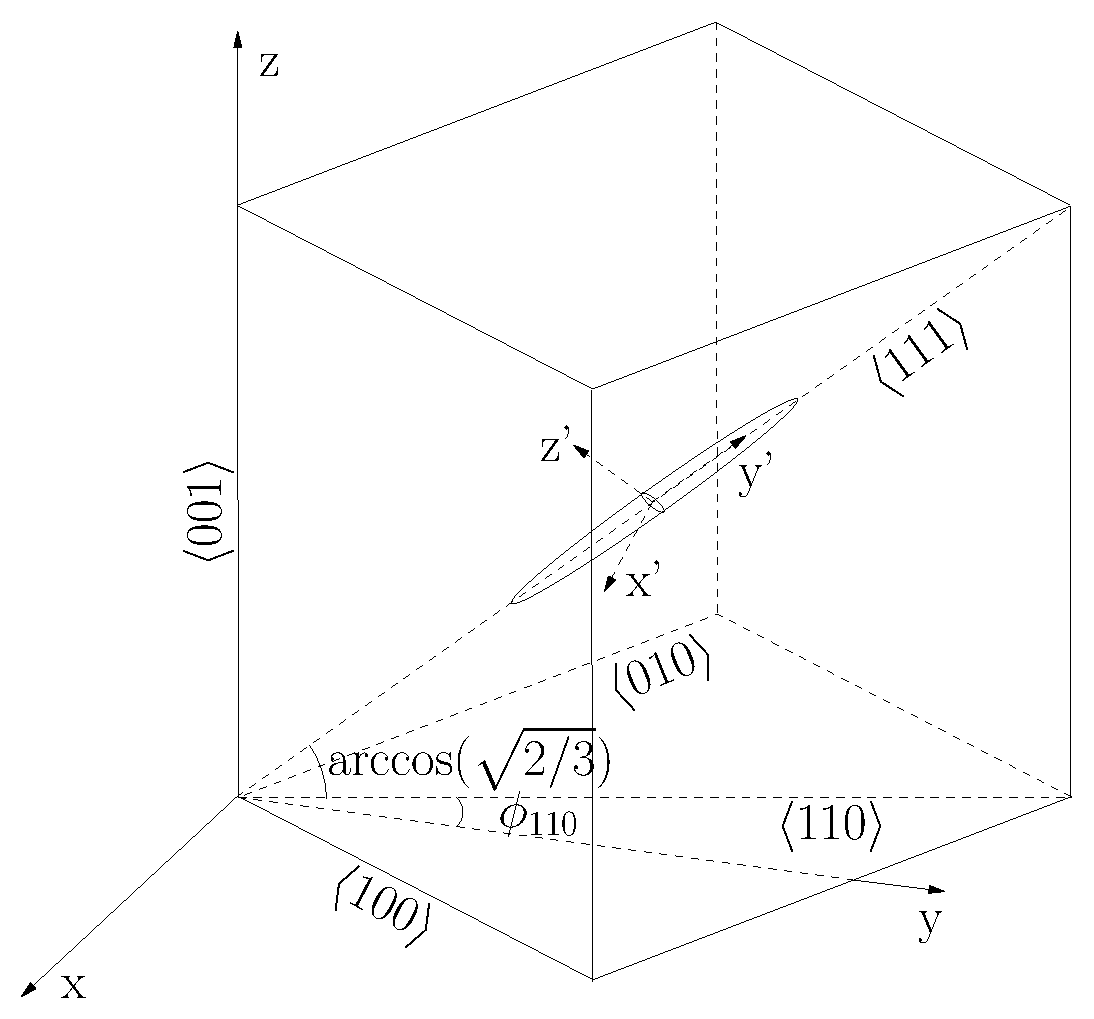
\includegraphics[width=0.4\textwidth]{axes}   
\caption{Relation between the local coordinates
$x^{\prime}y^{\prime}z^{\prime}$ in one of the four ellipsoidal
regions with conduction band valleys and the Geant4 coordinates
$xyz$. The $x^{\prime}$ axis is perpendicular to the plane defined by
$\langle111\rangle$ and $\langle001\rangle$.}
\label{fig:pss:axes} 
\end{SCfigure} 
 
The deviation from an equal population , i.e. $n_{e}/n$=1/4, of
electrons is assumed to depend on the electric field like:
\begin{equation} 
\label{eq:pss:nion} 
\frac{n_{j}}{n} = \mathcal{R}(E) \left[ \frac{\sqrt{\mathbf{E_{0}}\gamma_{j}\mathbf{E_{0}}}} 
{\sum_{i}\sqrt{\mathbf{E_{0}}\gamma_{i}\mathbf{E_{0}}}} - \frac{n_{e}}{n} \right] + \frac{n_{e}}{n},  
\end{equation} 
where the coefficient $\mathcal{R}$ is a function of $E=|\mathbf{E}|$
and the temperature.
 
An electric field applied along the $\langle 100 \rangle$ direction,
\textit{i.e.} $\mathbf{E_{0}} = (\sqrt{1/2}, \sqrt{1/2}, 0)^{T}$ in
$xyz$ coordinates affects the population of the electrons in all
$\langle 111 \rangle$ valleys equally, hence $n_{1}/n = n_{2}/n =
n_{3}/n = n_{4}/n = 1/4$. Using the drift velocity $v_{e}^{100}(E)$
according to Eq.~\ref{eq:pss:para}, the absolute value of
$\mathcal{A}(E)$ can be expressed as
\begin{equation} 
\label{eq:pss:ae} 
|\mathcal{A}(E)| = \frac{v_{e}^{100}(E)}  {\displaystyle \sum_{j} \frac{1}{4} \frac{\gamma_{j}\mathbf{E_{0}}} {\sqrt{\mathbf{E_{0}}\gamma_{j}\mathbf{E_{0}}}}}, \mbox{ with } \mathbf{E_{0}} = \left( \begin{array}{c}  
\sqrt{1/2}\\\sqrt{1/2}\\0 \end{array} \right). 
\end{equation} 
 
If the electric field vector is oriented along one of the four
$\langle 111 \rangle$ axes, \textit{i.e.} $\mathbf{E_{0}} = (0,
\sqrt{2/3}, \sqrt{1/3})^{T}$ in $xyz$ coordinates, there is an uniform
population of the electrons among the other three $\langle 111
\rangle$ axes, \textit{i.e.}
\begin{equation} 
\label{eq:pss:n111} 
\frac{n_{2}}{n} = \frac{n_{3}}{n} = \frac{n_{4}}{n}. 
\end{equation} 
Since 
\begin{equation} 
\label{eq:pss:nsum} 
\displaystyle \sum_{j}\frac{n_{j}}{n} = 1, 
\end{equation} 
we have 
\begin{equation} 
\label{eq:pss:n12} 
\frac{n_{1}}{n} + 3\frac{n_{2}}{n}= 1. 
\end{equation} 
Using the drift velocity $v_{e}^{111}(E)$ for an applied electric
field $E$ in the $\langle 111 \rangle$ direction at a specific
temperature according to Eq.~\ref{eq:pss:para}, another relation
between $n_{1}/n$ and $n_{2}/n$ is obtained:
\begin{equation} 
\label{eq:pss:n12p} 
v_{e}^{111}(E) =  \mathcal{A}(E) \left(  \frac{n_{1}}{n} \frac{\gamma_{1}\mathbf{E_{0}}}         {\sqrt{\mathbf{E_{0}}\gamma_{1}\mathbf{E_{0}}}} +  3\frac{n_{2}}{n} \frac{\gamma_{2}\mathbf{E_{0}}}         {\sqrt{\mathbf{E_{0}}\gamma_{2}\mathbf{E_{0}}}} \right). 
\end{equation} 
The values of $n_{1}/n$ and $n_{2}/n$ can be obtained by solving the
equations \ref{eq:pss:n12} and \ref{eq:pss:n12p}. Then
$\mathcal{R}(E)$ can be calculated as
\begin{equation} 
\label{eq:pss:re} 
\mathcal{R}(E) = \left( \frac{n_{1}}{n} - \frac{n_{e}}{n} \right) / \left( \frac{\sqrt{\mathbf{E_{0}}\gamma_{1}\mathbf{E_{0}}}} 
{\sum_{j}\sqrt{\mathbf{E_{0}}\gamma_{j}\mathbf{E_{0}}}} - \frac{n_{e}}{n} \right), \mbox{ with } \mathbf{E_{0}} = \left( \begin{array}{c}  
0\\ \sqrt{2/3}\\\sqrt{1/3} \end{array} \right). 
\end{equation} 
 
After the determination of the coefficients $\mathcal{A}$ and
$\mathcal{R}$ the drift velocity can be calculated for any direction
and any strength of the electric field. Figures~\ref{fig:pss:vvse}a
and c present the calculated electron drift velocities along the
$\langle 110 \rangle$ axis. The velocities are between the ones for
the other axes.

 
\subsection{Hole drift velocity} 
\label{sec:pss:hole} 
The model used to calculate the hole drift velocity is taken from
Ref.~\cite{bart}. In this model only the \emph{heavy hole valence
band} is responsible for the anisotropy of the mobility. All other
effects are neglected. A hole is accelerated by the electrical field
until its energy becomes 0.037~eV. At this point it is very likely to
emit an optical phonon and lose most of its energy, after which
acceleration in the field direction resumes and a new cycle starts.
 
The probability of finding a heavy hole in a specific momentum state
$\mathbf{k}$ is maximal in the direction parallel to the electric
field. The mean wave vector $\mathbf{k}_{0}(k_{0}, \theta_{0},
\phi_{0})$ is then assumed to be aligned with the electric field
$\mathbf{E}(E, \theta, \phi)$, \textit{i.e.} $\theta_{0} = \theta,
\phi_{0} = \phi$, where $\theta, \phi$ are the polar and azimuthal
angles with respect to the coordinate system defined by the $\langle
100 \rangle$, $\langle 010 \rangle$ and $\langle 001 \rangle$ axes as
shown in Fig.~\ref{fig:pss:vsphere}.
 
\begin{SCfigure}[][tbhp] 
\centering 
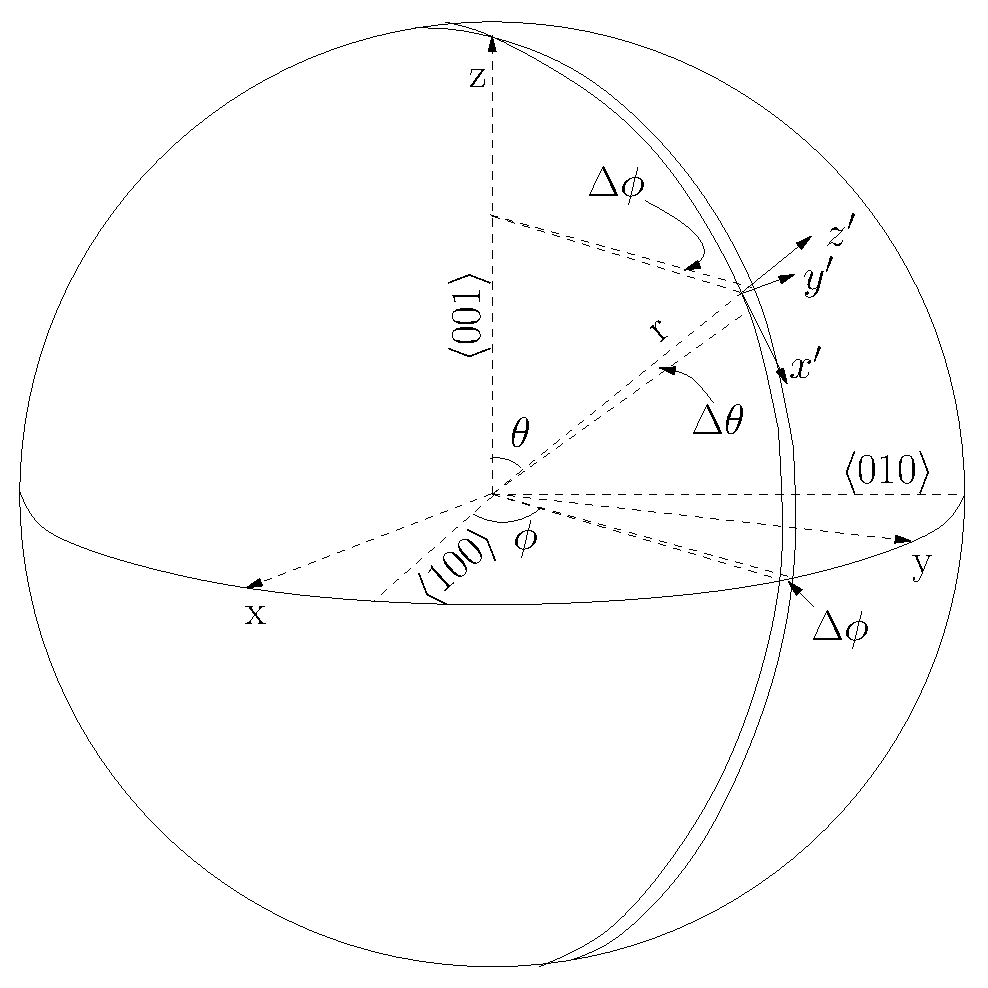
\includegraphics[width=0.4\textwidth]{vsphere}   
\caption{Relation between the crystal axes $\langle100\rangle$,
$\langle010\rangle$ and $\langle001\rangle$, and the coordinates $xyz$
used in Geant4, and the local coordinates
$x^{\prime}y^{\prime}z^{\prime}$.}
\label{fig:pss:vsphere} 
\end{SCfigure} 
 
The three components $(v_{x^{\prime}}, v_{y^{\prime}},
v_{z^{\prime}})^{T}$ of the hole drift velocity $\mathbf{v}$ in the
local coordinates, $x^{\prime}y^{\prime}z^{\prime}$, at any position
$(r, \theta, \phi)$ (as shown in Fig.~\ref{fig:pss:vsphere}) can be
expressed as:
\begin{equation} 
\label{eq:pss:vsphere} 
\begin{array}{rcl} 
v_{x^{\prime}} = v_{r} &=& v^{100}_{h}(E)[1-\Lambda(k_{0})(\sin(\theta)^{4}\sin(2\phi)^{2} + \sin(2\theta)^{2})],\\ 
v_{y^{\prime}} = v_{\theta} &=& v^{100}_{h}(E)\Omega(k_{0})[2\sin(\theta)^{3}\cos(\theta)\sin(2\phi)^{2} + \sin(4\theta)],\\ 
v_{z^{\prime}} = v_{\phi} &=& v^{100}_{h}(E)\Omega(k_{0})\sin(\theta)^{3}\sin(4\phi), 
\end{array} 
\end{equation} 
The mean wave number $k_{0}$ can be expressed as a function of
$v_{rel} = v^{111}_{h}(E)/v^{100}_{h}(E)$:
\begin{equation} 
\label{eq:pss:k0} 
k_{0}(v_{rel}) = 9.2652 - 26.3467v_{rel} + 29.6137v_{rel}^{2} - 12.3689v_{rel}^{3}, 
\end{equation} 
where $v^{111}_{h}(E)$ and $v^{100}_{h}(E)$ are the drift velocities
along the $\langle111\rangle$ and $\langle100\rangle$ axes. They can
be calculated using Eq.~\ref{eq:pss:para}. The magnitude of the
anisotropies, $\Lambda$ and $\Omega$, can be expressed as
\begin{equation} 
\label{eq:pss:lamb} 
\Lambda(k_{0}) = -0.01322k_{0} + 0.41145k_{0}^{2} - 0.23657k_{0}^{3} + 0.04077k_{0}^{4}, 
\end{equation} 
\begin{equation} 
\label{eq:pss:ome} 
\Omega(k_{0}) = 0.006550k_{0} - 0.19946k_{0}^{2} + 0.09859k_{0}^{3} - 0.01559k_{0}^{4}. 
\end{equation} 
 
The three components $(v_{x}, v_{y}, v_{z})^{T}$ of the hole drift
velocity $\mathbf{v}$ in $xyz$ coordinate (as shown in
Fig.~\ref{fig:pss:vsphere}) become:
\begin{equation} 
\label{eq:pss:v2v}   
\left( 
\begin{array}{c} 
v_{x} \\ v_{y} \\ v_{z} 
\end{array} 
\right) = R_{z}(\phi + \frac{\pi}{4} + \phi_{110}) R_{y^{\prime}}(\theta) \left(  
\begin{array}{c} 
v_{x^{\prime}} \\ v_{y^{\prime}} \\ v_{z^{\prime}} 
\end{array} \right), 
\end{equation} 
where $R_a(\alpha)$ indicates the counter-clockwise rotation around
the axes $a$ by the angle $\alpha$.  Figures~\ref{fig:pss:vvse}b and d
present the calculated hole drift velocities along the $\langle 110
\rangle$ axis. The velocities are between the ones along the other
axes.
 
 
\section{Drift trajectories } 
\label{sec:pss:trj} 
The trajectories are calculated iteratively.  The displacement vector
$\Delta \mathbf{r}$ by which a charge carrier drifts within a short
time interval $\Delta t$ can be calculated once the drift velocity
vector $\mathbf{v}_{i}$ in the original position $\mathbf{r}_{i}$ is
calculated using the method described in the previous two sections.
The new position $\mathbf{r}_{i+1}$ is then
\begin{equation} 
\label{eq:pss:pos} 
\mathbf{r}_{i+1} = \mathbf{r}_{i} + \Delta \mathbf{r} \ \ (i=0,1,...), \text{ with } \Delta \mathbf{r} = \mathbf{v}_{i} \Delta t. 
\end{equation} 
The iteration continues until the charge carriers reach the boundary
of the crystal. The series of position vectors $\mathbf{r}_{i}$ from
$\mathbf{r}_{0}$ to $\mathbf{r}_{\text{boundary}}$, $(\mathbf{r}_{0},
\mathbf{r}_{1}, ..., \mathbf{r}_{i}, ...,
\mathbf{r}_{\text{boundary}})$, represents the trajectory.
 
Two different numerical methods were used to calculate the trajectory,
the Euler method and the 4$^{th}$ Runge-Kutta method.  The Euler
method is less computer time intensive, but is also less precise.
However, for time intervals $\Delta t < 1$~ns, the output of the two
methods does not differ significantly.  The results presented here
were obtained with the Runge-Kutta method.
 
Figure~\ref{fig:pss:trjs} shows the drift trajectories projected on an
x-y cross sections of a Siegfried-like detector.  The crystal axis
$\langle 110 \rangle$ is assumed to be parallel to the x-axis
(\textit{i.e.}, $\phi_{110}$ as shown in Fig.~\ref{fig:pss:coo} is set
to zero). The left plot shows the inward drift of electrons starting
at the outer surface of the detector. The starting points are
distributed equidistantly on the outer circle.  The right plot shows
the outward drift of holes starting at the inner surface.  The
starting points are distributed equidistantly on the inner circle.
The bias voltage was set to 3000~V. The time interval was 1~ns.  The
time window for the calculation was 400~ns.  All electrons reach the
inner surface within this time window, but not all holes reach the
outer surface.  This is because electrons drift faster than holes.
Holes drift slowest along the $\langle 110 \rangle$ direction, as also
shown in Fig.~\ref{fig:pss:vvse}.
\begin{figure}[tbhp] 
\centering 
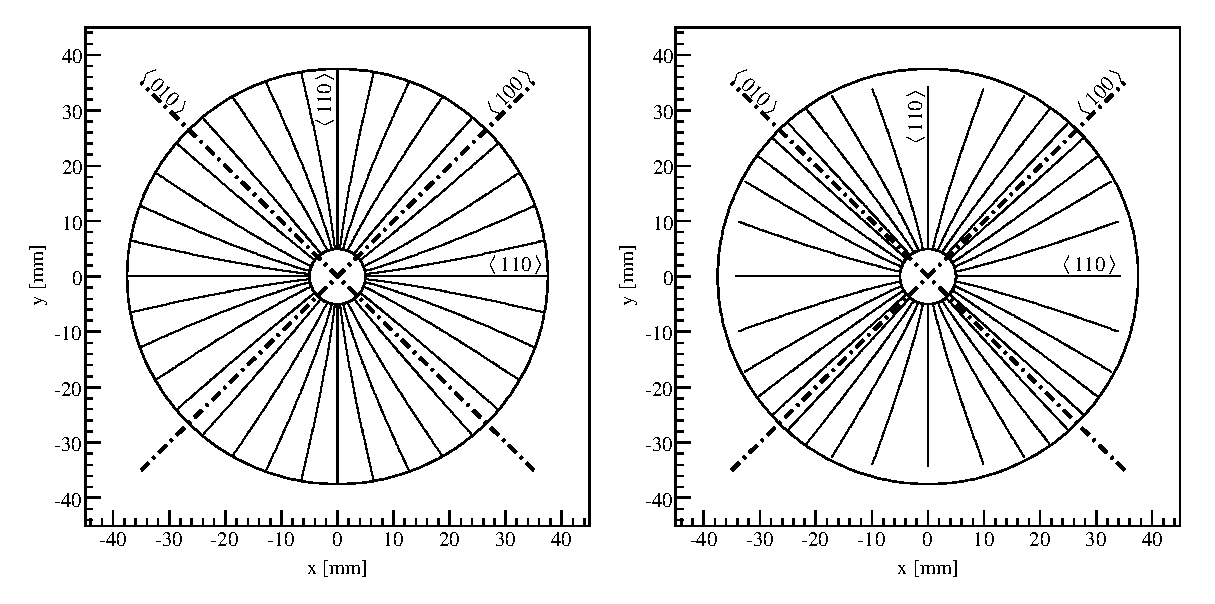
\includegraphics[width=\textwidth]{trjs} 
\caption{Drift trajectories projected on the x-y cross sections of
Siegfried-like detectors: Left, electrons drift inward; Right, holes
drift outward.}
\label{fig:pss:trjs} 
\end{figure} 
 
The trajectories along the crystal axes are straight as explained in
Sec.~\ref{sec:pss:mobi}.  However, they are clearly bent along other
directions.  This causes the different occupancies in different
segments that was shown in Fig.~\ref{fig:ph:mcb}.  The crystal axis
orientation can be deduced by comparing the occupancy distributions of
data and MC.  This will be described in detail in
Chapter~\ref{cha:psa}.
 
 
\section{Raw pulse shapes} 
\label{sec:pss:ps} 
Once the weighting fields and potentials as well as the drift
velocities and trajectories of the charge carriers are known,
Eq.~\ref{eq:det:ramoq} and \ref{eq:det:ramoi} introduced in
Sec.~\ref{sec:det:ramo} can be used to calculate the time development
of the induced charge $Q(t)$ or current $I(t)$ in each electrode (raw
pulses in short).  Figure~\ref{fig:pss:psh} shows the weighting
potential of a segment with the indication of an event.
Figure~\ref{fig:pss:pss} shows the raw charge and current pulses
induced by the resulting hit in this particular segment, its
neighboring segments and the core of a Siegfried-like detector.  The
amplitude of the pulse induced in one neighboring segment is larger
than in the other, because the trajectory of the hit is closer to this
segment.
\begin{figure}[htbp] 
\centering 
\subfloat[]{\label{fig:pss:psh} 
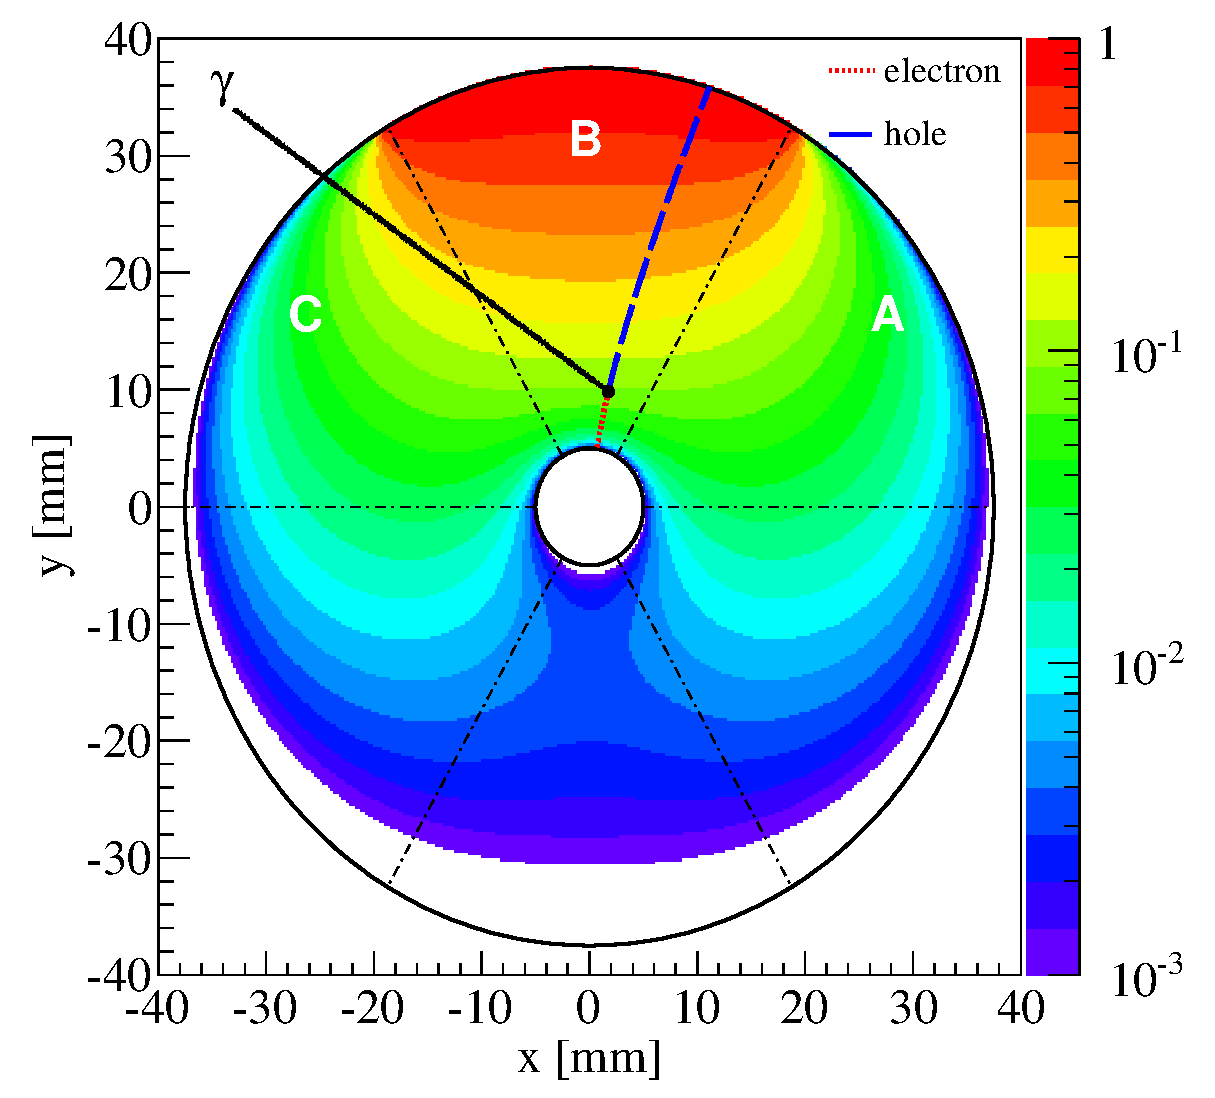
\includegraphics[height=0.22\textheight]{WP}}% 
\subfloat[]{\label{fig:pss:pss} 
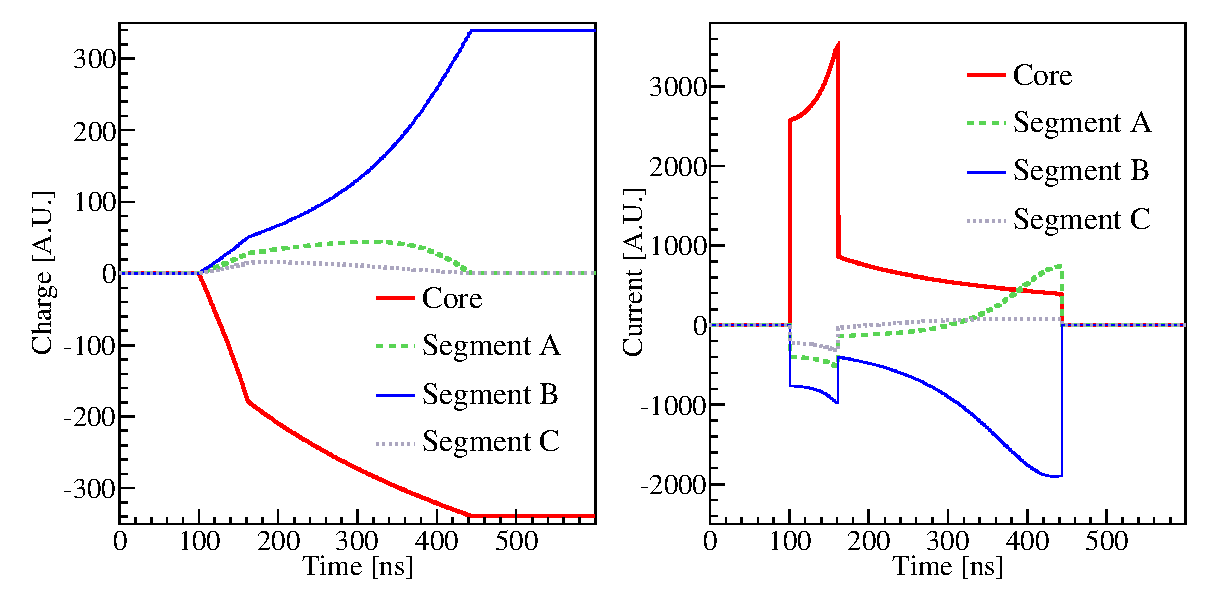
\includegraphics[height=0.22\textheight]{CIPS}}% 
\caption{(a) weighting potential of segment B together with an
indication of a $\gamma$ interaction. (b) Simulated charge and current
pulses induced in segments A, B and C.}
\label{fig:pss:ps} 
\end{figure} 
 
 
\section{Effects of electronics} 
\label{sec:pss:dbn} 
The pulses recorded by the DAQ system are quite different from the raw
pulses.  Not only their amplitudes but also their shapes are changed
by the electronics.  The baseline after a pulse exponentially
decreases to its original level with a time constant $\tau$. The limit
on the bandwidth of the signal transmission through the electronics
cuts off the signal components with frequencies higher than the
limit. Sharp edges in a pulse are hence smeared. Electronic noise may
destroy any detailed structure of a pulse.  All these effects need to
be simulated.
 
Figure~\ref{fig:pss:elec} shows a modified pulse after folding in the
decay of the baseline, the limited bandwidth and the noise. The decay
time was $5 \mu$s, the cut-off in bandwidth was 10~MHz and the noise
level was 5\% of the pulse amplitude. These values are worse than
observed in the tests tands. They were chosen to clearly demonstrate
influence of the effects.
\begin{figure}[htbp] 
\centering 
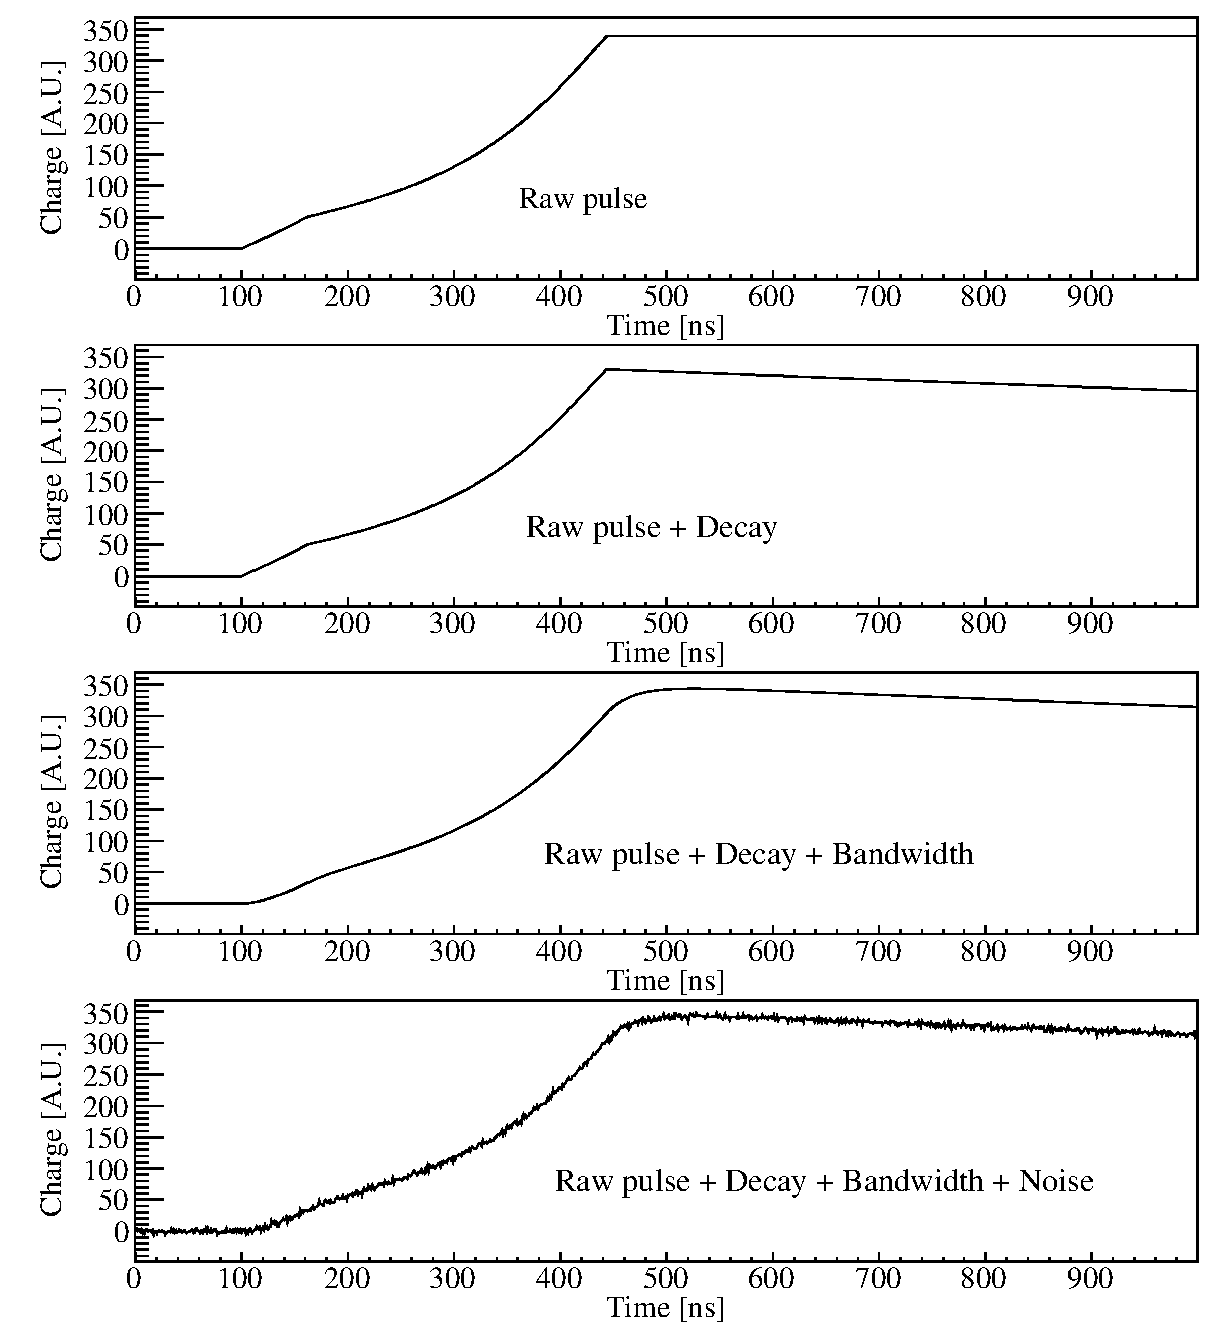
\includegraphics[width=0.7\textwidth]{PSDBN} 
\caption{Modified pulses after folding in the decay of the baseline,
the limited bandwidth and the noise.}
\label{fig:pss:elec} 
\end{figure} 
 
 
%%% Local Variables: 
%%% mode:latex 
%%% TeX-master: "thesis" 
%%% End: 
